\subsection{Data Collection}
For the data collection, a barebones Android app was developed, which reads the triaxial accelerometer and gyroscope data at a constant rate of 50hz along with a timestamp for each entry 
for simplification of signal processing. This was then exported as JSON format, and transferred to a computer. There was also an option to change the label before 
starting a recording session, where the folder would be named accordingly. This simplified the data set creation as we did not have to worry about labelling the data 
afterwards.\\
Using this app, several activities were carried out and recorded, whilst trying to vary the conditions as much as possible, such as putting it in the left and right pockets and having it upside down or upright, aiming to diversify the data.  
\begin{figure}[htp]
    \centering
    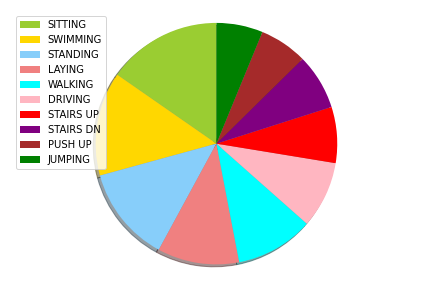
\includegraphics[width=.36\textwidth]{ethan_data_dist_pie}
    \caption{Our Data Distribution}
    % \label{fig:figureX}
    \label{our_data_count_dist}
    \end{figure}

Figure \ref{our_data_count_dist} depicts the different amounts of data collected per activity. Unfortunately, there was a considerable difference in the amount of data per activity, where some activities such as jumping had much less data than an activity like walking. This can lead to the accuracy of classification of data being misleading as if the classifier randomly guesses walking, it is right more times than if it randomly guesses jumping. 

\subsection{Signal Processing}
The JSON data exported from the mobile application was then ready to be imported by a python preprocessor. As is, the data is not usable by the classifiers, not only does it contain a lot of noise, but a single entry gives very little information about what is happening.\\
Consequently, several steps were to maximise the usability and the potential for classification of the data, such as synchronisation of gyroscope and accelerometer signals, use of a sliding window to group data, signal filtering and feature extraction using several statistical measures.   

\subsection{Synchronisation}
Due to a limitation from the application, the gyroscope and accelerometer collections worked asynchronously, and thus the entries were likely not to be aligned properly (few ms differences). And if the phone screen was turned off, data collection would stop and restart when the screen is turned on, which would cause a substantial gap within the data of a session.\\
A moving average of the differences was calculated over all the data. If the average is below 10ms, the values would be considered as forming part of the same timestamp, whilst if the average value was larger, an entry was removed from the accelerometer and gyroscope data, until the average restabilized. Thie eliminates most outliers, and if there are antired out of synch by a substantial margin, they are removed. This was considered quite harshly, as several techniques such as Fast Fourier transform rely on constant frequencies to provide desirable outputs. 
The first and last 2 seconds were also removed for each session, as time needs to be accounted for whilst the user puts the device in his/her pocket, which would provide inaccurate data. 


\subsection{Sliding Window}
As carried out int [https://www.sciencedirect.com/science/article/abs/pii/S1574119216302280] a sliding window was used to ‘group’ of size 128 with a stride of 64 (taking 128 entries (2.56 seconds of data) for each window, and overlap each window by 1.28 seconds).\\
This is one of the most crucial steps for data processing, as one single entry does not describe a whole lot about what a user is doing. Before any preprocessing, each entry simply has six values (two triaxial vectors), which are at a single point in time. When the sliding window is introduced, we group a window’s worth of entries into one, out of which we get a representation of what happens over a period (2.56 seconds in our case), where each window will represent 128 raw entries, containing 6 features (triaxial data) each. Which when feature mapped, summarizes features of this two-dimensional data frame, back into a one-dimensional entry, whilst still retaining the fact that an entry has now the added dimension of time.

\subsection{Signal Filtering}
A set of steps was applied to each window of entries, which will filter and prepare the data for the feature extraction.\\
\subsubsection{A low-pass Butterworth filter with a corner frequency of 20hz}
This removes most of the noise, as most changes in the acceleration happened at much lower frequencies, and through this separation, the most relevant changes in acceleration were kept. In fact according to [D.M. Karantonis, M.R. Narayanan, M. Mathie, N.H. Lovell, and B.G. Celler. Implementation of a
real-time human movement classifier using a triaxial accelerometer for ambulatory monitoring. IEEE
Transactions on Information Technology in Biomedicine, 10(1):156–167, 2006.] most bodily movements are contained below 15Hz

\subsubsection{Another low pass Butterworth filter was applied with a corner frequency of 0.3hz}
This filter separates gravitational acceleration from body acceleration, since changes in gravitational acceleration happen relatively slowly, a low corner frequency can distinguish and extract these changes as gravitational acceleration. 
\begin{figure}[htp]
    \centering
    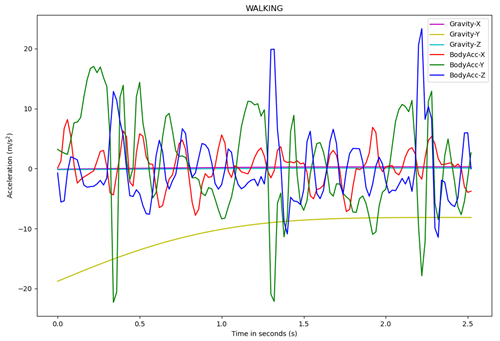
\includegraphics[width=.49\textwidth]{ethan_window_acc_plot}
    \caption{The Acceleration in a single window}
    \label{fig:figure_single_wind}
    % \label{fig:single_window_accels_out_data}
    \end{figure}

Figure \ref{fig:figure_single_wind} shows the 
different forces of acceleration experienced were plotted.
The Body forces show the filtered acceleration when separated from 
the gravitational acceleration. At idle, these forces should be zero. 
The strides of the walking may also be seen as the green line fluctuates, quickly 
dropping when the wearer’s foot descends and hits the floor. The other three stable plots are 
the gravitational forces experienced, these should not change as much, as the gravitational 
force experienced do not change much. At idle the vector of these three forces should point 
downwards with a magnitude of \textasciitilde $9.81m/s^2$.

\subsubsection{The Jerk was Calculated}
Jerk is defined as the change in acceleration and was calculated by differentiating the acceleration values by time(1/(50hz)=0.02s). This gives a better idea of how drastically the accelerations change, such as when one is jogging and the leg where the phone is sitting stops sharply as it hits the ground.

\subsubsection{The Magnitude}
The magnitude is the measure of how much the values differ from zero. This comes useful when one simply needs an idea of the amount of force applied, without considering the effects of directionality.

\subsubsection{Fast Fourier Transform}
FFT enabled the calculation of frequency components based on the time-varying signals. When considering Human Activity, one can note that there is a lot of repetitive patterns, in which case transformations such as FFT are used to calculate the discrete Fourier transform, and give a rich statistic for summarizing a window of these repetitive signals.
\\
\[https://www-proquest-com.ejournals.um.edu.mt/docview/2301775170/fulltextPDF/431219E14EB34859PQ/1?accountid=27934\]



\subsection{Feature Extraction}
    Excluding the label for each activity, each session in the dataset contains 589 features. These features were extracted by applying a number of different statistical
    measures to the different extracted signals in each sliding window.

    Each signal has the statistical measures in Table 1 applied to them.

    \begin{table}[ht]
        \begin{tabular}{|l|l|lll}
            \cline{1-2}
            \textbf{Statistical Measure} & \textbf{Description} &  &  &  \\ \cline{1-2}
            mean             & Mean value in the window           &  &  &  \\ \cline{1-2}
            min            & Smallest value in the window           &  &  &  \\ \cline{1-2}
            max            & Largest value in the window           &  &  & \\ \cline{1-2}
            std            & Standard deviation           &  &  & \\ \cline{1-2}
            entropy            & Entropy           &  &  & \\ \cline{1-2}
            mad            & 3           &  &  & \\ \cline{1-2}
            iqr            & Inter-quartile Range           &  &  & \\ \cline{1-2}
            energy            & 3           &  &  & \\ \cline{1-2}
            sma            & Signal magnitude area           &  &  & \\ \cline{1-2}
            arCoeff            & 3           &  &  & \\ \cline{1-2}
            correlation            & 3           &  &  & \\ \cline{1-2}
            angle            & Angle between 2 vectors of signals           &  &  & \\ \cline{1-2}
            band energy            & 3           &  &  & \\ \cline{1-2}
        \end{tabular}
        \caption*{Table 1}
    \end{table}

    The statistical measures in Table 2 are applied only to FFT signals.

    \begin{table}[ht]
        \begin{tabular}{|l|l|lll}
            \cline{1-2}
            \textbf{Statistical Measure} & \textbf{Description} &  &  &  \\ \cline{1-2}
            maxInds             & 1           &  &  &  \\ \cline{1-2}
            skewness            & 2           &  &  &  \\ \cline{1-2}
            kurtosis               & 3           &  &  &  \\ \cline{1-2}
            meanFreq            & 3           &  &  &  \\ \cline{1-2}
        \end{tabular}
        \caption*{Table 2}
    \end{table}


\subsection{Signal Processing}

\subsection{Support Vector Classifier}
    \subsubsection{Data Pre-processing}
        Firstly, the training and testing datasets were converted to Pandas dataframes and the labels for each activity were separated into their own variables.
        Using a LabelEncoder, each activity label is converted into a numerical value.

    \subsubsection{Comparing different classification models}
        In total, four different classic machine learning classifiers were used on the dataset developed by Anguita et al \cite{Anguita2012}. These classifiers are Gaussian Naïve Bayes,
        AdaBoost, Stochastic Gradient Descent and a Support Vector Classifier. These were trained and tested using the respective datasets, and their accuracy,
        F-beta, precision and recall scores were recorded.

        \begin{table}[ht]
            \centering\footnotesize
            \begin{tabular}{|l|l|l|l|l|}
                \hline
                \textbf{Classifier} & \textbf{Accuracy} & \textbf{F-Beta}  & \textbf{Precision} & \textbf{Recall} \\ \hline
                Gaussian Naïve Bayes             & 0.7134           & 0.7252  & 0.7555 & 0.7134 \\ \hline
                AdaBoost            & 0.4065           & 0.2520 & 0.4289 & 0.4065 \\ \hline
                Stochastic Gradient Descent               & 0.9600           & 0.9603 & 0.9605 & 0.9600 \\ \hline
                Support Vector Classifier            & 0.9668           & 0.9676 & 0.9682 & 0.9668 \\ \hline
            \end{tabular}
            \caption*{Table 3: Performance scores of each classifier}
        \end{table}

        As can be seen in Table 3, the Support Vector Classifier had the highest scores, each result being over 0.96. It is for this reason that the SVC
        was chosen to classify the UCI dataset \cite{Anguita2013} and, later on, the dataset built by ourselves.

    \subsection{Classification}
        The RBF kernel is defined as the exponential function \(exp(-\gamma \lvert x-x' \rvert)^2\) A primer on kernel methods, JP Vert et al, where x and x’ are two feature vectors, and is the
        gamma parameter in the classifier. Gamma’s value is scale, meaning that the parameter is the reciprocal of the number of features multiplied with the variance of the input data.
        For this implementation, we opted for a One-Vs-All approach. A One-Vs-All approach divides the data points into just two classes: a certain activity X and the other classes. Therefore records
        labelled as \emph{SITTING} are a single class, and the other activities are treated as having a single label.

\subsection{Convolutional Neural Network}
    In the research done numerous CNN implementations designed for the UCI dataset like [include numerous] were checked.
    From these, [paper] presented the choice and implementation of a CNN use for HAR the best.
    Hence, the implementation described in this report is based on the architectures described in [the paper].
    Unlike [paper authors] we did not  implement a first stage dynamic-static split model and instead opted to split the labels manually.
    The Pytorch [reference it] library was used to implement the CNNs, and the sklearn [reference it] library to evaluate the results.

    \subsubsection{Data Split}
        The train/valid/test split was an 80/20 train/test split, then 80/20 train/validation split for the UCI dataset, and a 90/10 train/test split, then 90/10 train/validation split for Our Dataset.
    \subsubsection{Dataset Object}
        To facilitate this dynamic/static split we defined a Python dictionary with each label having a number assigned to it, starting from 0.
        The numbering needs to start from 0 as the output of neural networks implemented in Pytorch always start from 0.
        Another requirement for implementing neural networks in Pytorch is to implement a custom Dataset object.
        The function of this object is to read the data from a source and define its X, data and Y, labels counterparts.
        The Pandas [reference it] library was used at this stage due to its use of the numpy [reference it] library and efficient data management.
        It is important that the X component is in the shape: length(data.columns), 1, length(data.rows)).

        The dataset object was initialised 3 times, for the Train, Validation and Testing data.

        The pie charts included below show the training, validation and testing label distribution in order.

        \begin{figure}[htp]
        \centering
        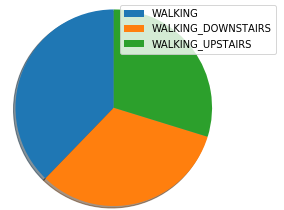
\includegraphics[width=.15\textwidth]{UCI_Dynamic_Training}\hfill
        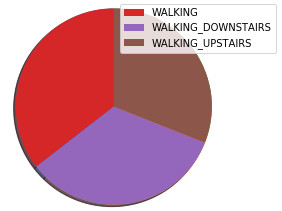
\includegraphics[width=.15\textwidth]{UCI_Dynamic_Validation}\hfill
        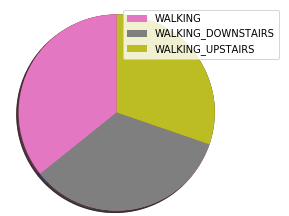
\includegraphics[width=.15\textwidth]{UCI_Dynamic_Testing}
        \caption{UCI Dynamic Label Distribution}
        \label{fig:figureX}
        \end{figure}

        \begin{figure}[htp]
        \centering
        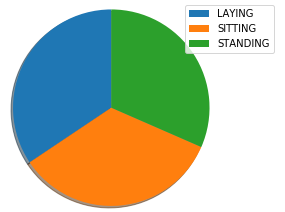
\includegraphics[width=.15\textwidth]{UCI_Static_Training}\hfill
        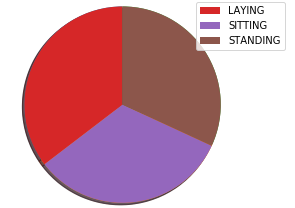
\includegraphics[width=.15\textwidth]{UCI_Static_Validation}\hfill
        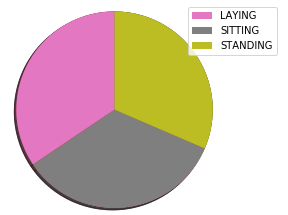
\includegraphics[width=.15\textwidth]{UCI_Static_Testing}
        \caption{UCI Static Label Distribution}
        \label{fig:figureX}
        \end{figure}

        \begin{figure}[htp]
        \centering
        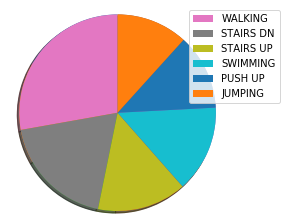
\includegraphics[width=.15\textwidth]{OD_Dynamic_Training}\hfill
        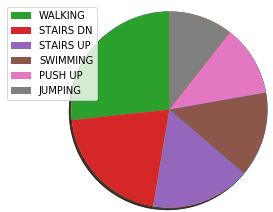
\includegraphics[width=.15\textwidth]{OD_Dynamic_Validation}\hfill
        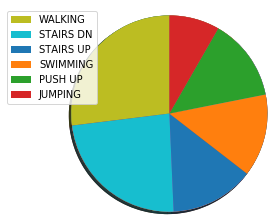
\includegraphics[width=.15\textwidth]{OD_Dynamic_Testing}
        \caption{OD Dynamic Label Distribution}
        \label{fig:figureX}
        \end{figure}

        \begin{figure}[htp]
        \centering
        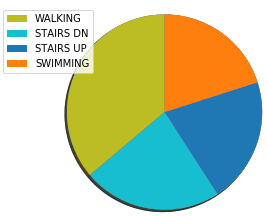
\includegraphics[width=.15\textwidth]{OD_Static_Training}\hfill
        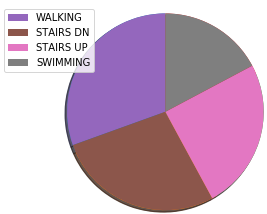
\includegraphics[width=.15\textwidth]{OD_Static_Validation}\hfill
        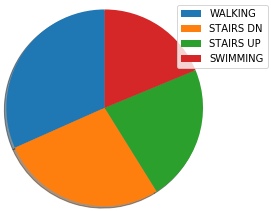
\includegraphics[width=.15\textwidth]{OD_Static_Testing}
        \caption{OD Static Label Distribution}
        \label{fig:figureX}
        \end{figure}

        In development, it was noted that the data distribution of the dynamic activities in our dataset was unequal.
        This was causing issues with the CNN's accuracy.
        To combat this added functionality was added with the aim of increase the quality of the model's output.
        In this project the number of rows for each eligible label was stored.
        Using the functionality provided by the Pandas library, the index for each label was stored in a list linked to its respective label.
        Using Python list slicing these lists where cut down to their lowest common length.
        These indices where then converted into a new Pandas dataframe and this balanced dataset was used for the dynamic model.

        \begin{figure}[htp]
        \centering
        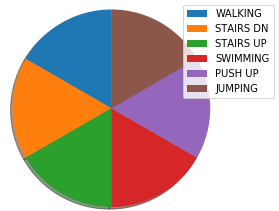
\includegraphics{OD_Dynamic_Training_Balanced}
        \caption{OD Dynamic Training Balanced Label Distribution}
        \label{fig:figureX}
        \end{figure}

        Finally the dataset objects are used to initialise a Dataloader object.
        This object gives us the functionality of delivering batches as inputs to the models at training and testing.
        It was found that a batch size of 32 worked best for the Static models, and a batch size of 64 worked best for the dynamic models.

    \subsubsection{Model Creation}
        The CNN models where implemented following the design of the below diagrams.
        Every model used the Cross Entropy as their loss function and the ADAM optimizer.
        The learning rate for the UCI Dataset Models, and Our Dataset Static model was set at 0.0005 and were trained for 10 epochs.
        The learning rate for the Our Dataset Dynamic model was set at 0.00005 and were trained for 11 epochs.